\section{Structural Design Patterns}

% Two columns start
\iftwocolumns
\begin{multicols}{2}
\fi

Structural design patterns are generally utilized to help organizing the structure and relationship of objects.

\subsection{Adapter}

An adapter is a structural design pattern that wraps an incompatible object such that it can be used/interfaced by the client.\cite{sm-adapter}. Such pattern is commonly used to integrate third party \textit{application program interface} (API) or libraries into the project. In other words, an adapter will take something that has already been designed or built that would not work with current solution, ``retrofit" around that and make unrelated classes work together.\cite{sm-adapter}\bs
\\
A middle layer that transforms the interface of a desired object (usually provided by libraries) to work with client.\bs
\\
An example used in game right now is adapting data from local client to an online database. Suppose we have some  player persistence data for an online game stored on a database in a form of a JSON object. When we fetch the player data from the server to be used in gameplay, the JSON object would need to be ``parsed'' to some usable object in C++. Thus an adapter would be used to read the JSON and populate another object with one-to-one mapping.\bs
\\
When we change the player data locally, we then need another adapter to serialize the data in the client player object to JSON such that it can be posted to the database again.\bs
\\
Another example would be adapting file formats such as 3D model objects and texture formats such as textures.\bs
\\
In appendix section \ref{code:adapter}, I demonstrate one of the simplest form of an adapter. Suppose we utilize a graphics library that has a rectangle drawing function that takes the parameter of \texttt{(int x, int y, int w, int h)} where they represent x-coordinate, y-coordinate, width, and height respectively. But our client code, instead of knowing the width and height of the rectangle, knows the x and y-coordinate of the opposite corner. Of course, the client could do the conversion itself, but the implementation could get more complex and repetitive as we deal with more complex interfaces.\bs
\\
In essence, the adapter design pattern is beneficial in game development to fit incompatible parts to the project. Thereby reduces development time that it would take for re-implementation.\bs
\\

\textbf{Difference Between Adapter and Mediator}\bs
\\

Note that adapters are different from \textit{mediators} (section \ref{ssection:mediator}), as mediator manages the communication between two classes, essentially decouples the interaction of the two. Whereas adapter simply translates.\bs
\\
Consider a real life analogy, where two people who speak different languages are fighting. A mediator would be a lawyer such that the two people don't talk to each other directly. An adapter would be a translator so that the two can communicate more directly. Thus, adapters are structural and mediators are behavioral.

\subsection{Bridge}
The \textit{bridge} pattern decouples abstraction from its implementation which enables orthogonal hierarchies. One could think of orthogonal hierarchies like orthogonal basis vectors from linear algebra. Using the basis vectors, we could construct any vector of the same domain using linear combination. Likewise for orthogonal hierarchies, the separation of interface and implementation allow us to have a combination of the different derived types.\bs
\\
The bridge patterns are notably used to encapsulate classes that would need to work on multiple platforms, which would require multiple implementations.\bs
\\
Consider a scenario where we have multiple types of subclasses that has an orthogonal property such as one depicted in figure \ref{fig:bridge-before}. Notice that if we were to add more types of guns or more gun attachments, the number of derived classes that need to be implemented grows geometrically. Resulting in highly un-maintainable and repetitive code.\bs
\\
Note that all the derived classes share some commonalities. In particular, any derived gun class inherits one of pistol, assault rifle, or LMG. And has modification of one of scope, suppressor, and ergonomic grip. By using the bridge pattern to decouple the implementation from the interface, we can make \textit{orthogonal hierarchies} (figure \ref{fig:bridge-after}) which is more manageable.\bs
\\

\iftwocolumns
\end{multicols}
\fi

\begin{figure}[H]
	\centering
	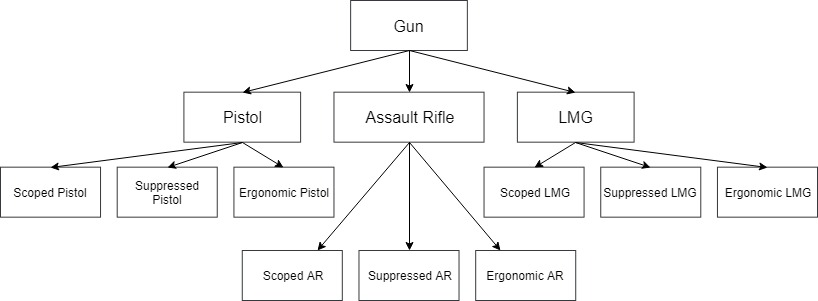
\includegraphics[width=0.8\textwidth]{assets/bridge-before}
	\caption{Structure of orthogonal hierarchy before using bridge pattern}
	\label{fig:bridge-before}
\end{figure}

\begin{figure}[H]
	\centering
	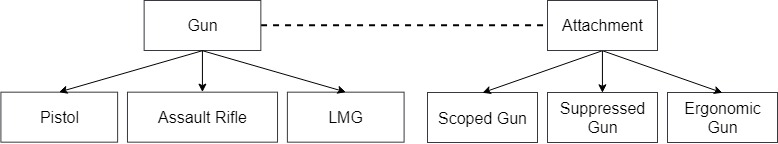
\includegraphics[width=0.75\textwidth]{assets/bridge-after}
	\caption{Structure of orthogonal hierarchy after using bridge pattern}
	\label{fig:bridge-after}
\end{figure}

\iftwocolumns
\begin{multicols}{2}
\fi

\subsection{Composite}
The composite design pattern allow objects to be composed into nested hierarchies or tree structures. The client can treat the composited object or the composition of objects the same way.\cite{sm-composite}.

\begin{figure}[H]
	\centering
	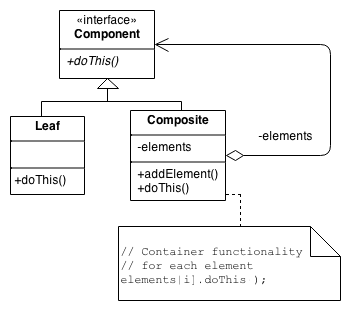
\includegraphics[width=0.4\textwidth]{assets/composite-sm}
	\caption{Simple structure of composite design pattern\cite{sm-composite}}
	\label{fig:composite}
\end{figure}

As seen in figure \ref{fig:composite}, the client would interact with the root interface \textit{Component}. The derived \textit{Composite} class holds a list of elements with the type \textit{Component} such that a recursive/tree-like structure could be constructed. Alongside, the the derived \textit{Leaf} class has more unique data and behaviors, but still desired to be part of the composition.\bs
\\
The result is that we can have nested relationships abstracted. The interface allows all nested classes to be treated the same by the client. Such as the example shown in figure \ref{fig:composite-arith} of a composited mathematical expression. Since the composite is recursive, the interface could expose a single call to the client to evaluate all children composites and leaf objects.\bs
\\
\begin{figure}[H]
	\centering
	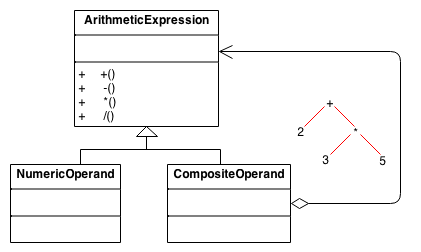
\includegraphics[width=0.4\textwidth]{assets/composite-arith}
	\caption{Composite pattern used for representing mathematical expression\cite{sm-composite}}
	\label{fig:composite-arith}
\end{figure}

The composite pattern is apparent in UI layouts. For instance, a standard desktop application window has the main window widget itself, but it has nested components inside it. These nested components are also sometimes expected to hold items inside themselves. As seen in figure \ref{fig:submenus}, the main window has a menu bar, the menu bar contains menu buttons which open to another list of menus and the nesting goes on.

\begin{figure}[H]
	\centering
	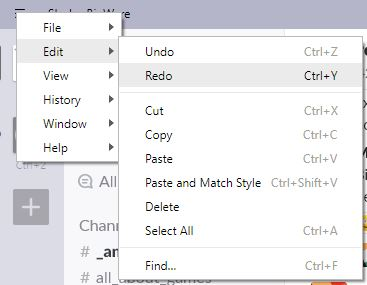
\includegraphics[width=0.4\textwidth]{assets/submenus}
	\caption{Composite pattern in menu systems in UI}
	\label{fig:submenus}
\end{figure}

Similar ideas apply to in-game UIs, where elements that composes the game UI are made of smaller components known as \textit{UIWidgets}. Designers put multiple UIWidgets together, sometimes reusing existing ones to create a screen of UI, as seen in figure \ref{fig:anthem-forge}.

\begin{figure}[H]
	\centering
	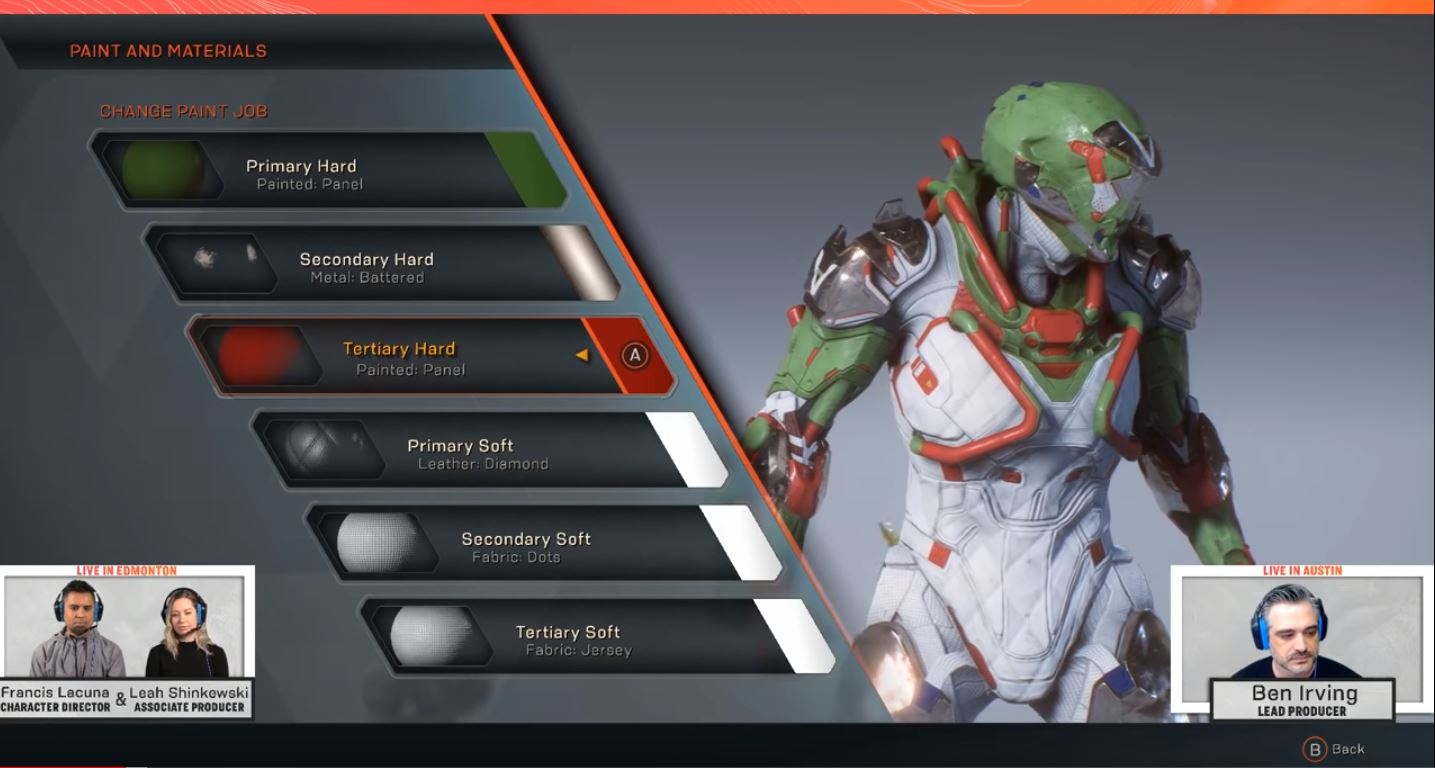
\includegraphics[width=\fullwidth]{assets/anthem-forge}
	\caption{UI menus in Anthem\cite{anthem-customization}}
	\label{fig:anthem-forge}
\end{figure}

% Useful in architectures such as component-entity-systems model which centers around the idea of ``\textit{composition over inheritance}" (section \ref{ssection:ecs}).

\subsection{Decorator}

Consider the following problem: suppose we have a ``gift'' class whose purpose is to hold some intrinsic information about the gift, such as what it is and its value (i.e. an avocado, with value of \$1.20). However, there exists times when we need to delegate responsibilities the \textit{gift} class dynamically (during run-time), such as concealing the gift value or wrapping the gift and putting it in a box. In this case, the wrappers and boxes would be extra responsibilities delegated to the gift. However, we would not want to define this statically as it is not flexible (what if we want to different wrapping paper depending on the recipent). Thus, it would be wise to utilize the decorator design pattern.\bs
\\
As the name suggests, the decorator design pattern ``decorates'' around the class that we want to assign new responsibilities to. To apply this pattern in software, we first create an \textit{interface class} that holds the lowest common denominator attributes and functions of the \textbf{core class} (the class that holds the core functionalities) and the \textbf{decorator class} (the class that decorates the core classes). We then create the \textit{decorator} base class that implements the interface a level down. The interface allows programmers to establish a loosely coupled relationship in code, and being a base class opens the option for more decorator variations.\bs
\\
Note that both \textit{core} and \textit{decorator} classes extends the interface via ``is a'' relationship. In addition, \textit{decorator} holds a memeber variable of the interface type. This way, the decorator classes can actually perform the tasks that delegates to the core classes or more decorator classes.\bs
\\
Lastly, the client is responsible for managing the creation of the decorators as well as the composition of the decorator classes added to the core classes.\bs
\\
In games, such pattern is applicable in game assets that have the ability to be modified. To name a few, these game objects could be potion effects to playable or non-playable characters (NPCs) (figure \ref{fig:minecraft-potion-effect}), modifications to vehicles (figure \ref{fig:bf4-vehicle-mods}), or enchantment on tools or weapons (figure \ref{fig:minecraft-enchantments}).\bs
\\
The decorator is a structural design pattern to enhance the flexibility of OOP software by allowing extra behaviors to be attached to the core class during run-time. The decoupling of core class functionalities from the potential (but optional) decorator functionalities reduces the tedious need of programming every permutation of core and decorator classes. Thus, the codebase is more maintainable as well. The decorator design pattern shows no change in performance.\bs
\\
Sample code for an exmaple of how the decorator pattern is used in a generic UI scenario is available in section \ref{code:decorator}.

\subsection{Facade}
TODO: Facade is a single class that represents an entire system which provides better separation and abstraction. Improves code maintainability and decouples critical parts of a system from external interactions

\subsection{Flyweight}
TODO: Flyweight are used to share expensive objects more efficiently. 

\subsection{Proxy}
TODO: Placeholder class to another class to control access to it. It provides an additional in-between level to support more controlled access. The proxy wraps the object and add delegation that matches the original class interface exactly (which is different from adapter, as adapter changes the interface). Examples include smart pointers, etc. (insert 4 common uses).


% Two columns end
\iftwocolumns
\end{multicols}
\fi